% \section{Generation of the Model Zoos}
\section{Model Zoo Generation}
\vspace{-1pt}
The proposed model zoo datasets contain systematically generated and diverse populations of neural networks.
Since the applicability of the model zoos for downstream tasks largely depends on the composition and properties 
of the zoos, special care has to be taken in their design and the used protocol for training. 
The entire procedure can be considered as defining and restricting the generating factors of
model zoo training with respect to their latent relation of desired zoo characteristics. 
%
The described procedure and protocol could be also used as general blueprint for the generation of model zoos.\looseness-1

% \paragraph{Definition} 
In our paper, the term architecture means the structure of a NN, i.e., set of operations and their connectivity. 
We use 'model' to denote an instantiating of an architecture with weights over all stages of training, 'model state' to denote the model with the specific state of weights at a specific training epoch, and the weights ${\textbf{w}}$ to denote all trainable parameters (weights and biases).\looseness-1
% , samples to denote weights of a given model. 

%%%%%%%%%%%%%%%%%%%%%%%%%%%%%%%%%%%%%%%%%%%%%%%%%%%%%%
%
%   the design, intention, and process
%
%%%%%%%%%%%%%%%%%%%%%%%%%%%%%%%%%%%%%%%%%%%%%%%%%%%%%%
\subsection{Model Zoo Design}
\label{sec:generation}

\vspace{-3pt}
\paragraph{Generating Factors}
Following~\citep{unterthinerPredictingNeuralNetwork2020}, we define the tuple $\{ \mathcal{D}, \lambda,  \mathcal{A}\}$ as a configuration of a model 
zoo's generating factors. We denote the dataset of image samples with their corresponding labels  as $\mathcal{D}$. 
The NN architecture is denoted by $\mathcal{A}$.
We denote the set of hyperparameters used for training, (\textit{e.g.}, loss function, optimizer, learning rate, weight initialization, seed, batch-size, epochs) as $\lambda$. 
% We define as $\mathcal{A}$, a specific NN architecture, which is used for all models of the model zoo.
While dataset $\mathcal{D}$ and architecture $\mathcal{A}$ are fixed for a model zoo, $\lambda$ provides not only the set of hyperparameters but also configures the ranges for individual hyperparameter such as learning rate for model zoo generation.
%
Training with such differing configurations $\{\mathcal{D}, \lambda,  \mathcal{A}\}$ results 
in a population of NN models i.e., the model zoo. We convert the weights and biases of each model 
to a vectorized form. In the resulting model zoo $\mathcal{W} = \{ {\textbf{w}}_1, ...., {\textbf{w}}_M \}$, ${\textbf{w}}_i$ 
denotes the flattened vector of the weights and biases of one trained 
NN model from the set of $M$ models of the zoo. \looseness-1

\vspace{-3pt}
\paragraph{Configurations \& Diversity}
% The model zoos have to be diverse enough but still suitable to be exploited for multiple downstream tasks. 
The model zoos have to be representative of real world models, but also diverse and span an interesting range of properties.
The definition of diversity of model zoos, as well as the choice of how much diversity to include, 
is as difficult as in image datasets, e.g.~\citep{dengImageNetLargeScaleHierarchical,feiConstructionAnalysisLarge}.
Model zoos can be diverse in their properties (i.e., performance) as well as in their generating factors $\lambda$, or in their weights $\textbf{w}$. 
% While all is desirable, the properties are indirectly controlled by the generating factors, which also determine the weights. 
We aim at generating model zoos with a rich set of models and diversity in these aspects.
As these zoo properties are effects of the generating factors, we tune the diversity of the generating factors 
and evaluate the diversity in Section \ref{sec:analysis}.

%
\begin{table}[]
\begin{tabular}{lllllllll}
\cline{1-8}
\end{tabular}
\end{table}

\begin{table}[]
{
\scriptsize
\caption{Generating factors of the model zoos. Several values for each parameter define the grid.
\texttt{Arch} denotes the architecture: CNN (s) - small CNN architecture, CNN (m) - medium CNN architecture, RN-18 - ResNet-18.
\texttt{Init} denotes the initalization methods: U - uniform, N - normal, KU - Kaiming Uniform, KN - Kaiming Normal.
\texttt{Activation} denotes the activation function: T - Tanh, S - Sigmoid, R - ReLU, G - GeLU.
\texttt{Optim} denotes the optimizer: AD - Adam, SGD - Stochastic Gradient Descent.
Models with learning rates denoted with * have been trained with a one-cycle LR scheduler, the listed LR is the maximum value.
}
\label{tab:generating_factors}
{
\centering
\begin{tabular}{@{}lllccccccc@{}}
\toprule
Dataset                        & Arch & Config & \texttt{Init}           & \texttt{Activation}     & \texttt{Otpim}     & \texttt{LR}        & \texttt{WD}              & \texttt{Dropout}       & \texttt{Seed}   \\
\cmidrule(r){1-1} \cmidrule(rl){2-2}  \cmidrule(rl){3-3} \cmidrule(rl){4-4} \cmidrule(rl){5-5}  \cmidrule(rl){6-6}  \cmidrule(rl){7-7}  \cmidrule(rl){8-8}  \cmidrule(rl){9-9} \cmidrule(rl){10-10} 
\multirow{3}{*}{MNIST}         & CNN (s) & Seed          & U              & T              & AD          & 3e-4      & 0             & 0           & 1-1000 \\
                               & CNN (s) & Hyp-10-r   & U, N, KU, KN & T, S, R, G     & AD, SGD     & 1e-3,1e-4 & 1e-3, 1e-4      & 0, 0.5      & $\sim 10$     \\
                               & CNN (s) & Hyp-10-f    & U, N, KU, KN & T, S, R, G     & AD, SGD     & 1e-3,1e-4 & 1e-3, 1e-4      & 0, 0.5      & 1-10   \\
\cmidrule(r){1-1} \cmidrule(rl){2-2}  \cmidrule(rl){3-3} \cmidrule(rl){4-4} \cmidrule(rl){5-5}  \cmidrule(rl){6-6}  \cmidrule(rl){7-7}  \cmidrule(rl){8-8}  \cmidrule(rl){9-9} \cmidrule(rl){10-10} 
\multirow{3}{*}{F-MNIST}       & CNN (s) & Seed          & U              & T              & AD          & 3e-4      & 0             & 0           & 1-1000 \\
                               & CNN (s) & Hyp-10-r   & U, N, KU, KN & T, S, R, G     & AD, SGD     & 1e-3,1e-4 & 1e-3, 1e-4      & 0, 0.5      & $\sim 10$        \\
                               & CNN (s) & Hyp-10-f    & U, N, KU, KN & T, S, R, G     & AD, SGD     & 1e-3,1e-4 & 1e-3, 1e-4      & 0, 0.5      & 1-10   \\
\cmidrule(r){1-1} \cmidrule(rl){2-2}  \cmidrule(rl){3-3} \cmidrule(rl){4-4} \cmidrule(rl){5-5}  \cmidrule(rl){6-6}  \cmidrule(rl){7-7}  \cmidrule(rl){8-8}  \cmidrule(rl){9-9} \cmidrule(rl){10-10} 
\multirow{3}{*}{SVHN}          & CNN (s) & Seed          & U              & T              & AD          & 3e-3      & 0             & 0           & 1-1000 \\
                               & CNN (s) & Hyp-10-r   & U, N, KU, KN & T, S, R, G     & AD, SGD     & 1e-3,1e-4 & 1e-3, 1e-4, 0 & 0, 0.3, 0.5 & $\sim 10$        \\
                               & CNN (s) & Hyp-10-f    & U, N, KU, KN & T, S, R, G     & AD, SGD     & 1e-3,1e-4 & 1e-3, 1e-4, 0 & 0, 0.3, 0.5 & 1-10   \\
\cmidrule(r){1-1} \cmidrule(rl){2-2}  \cmidrule(rl){3-3} \cmidrule(rl){4-4} \cmidrule(rl){5-5}  \cmidrule(rl){6-6}  \cmidrule(rl){7-7}  \cmidrule(rl){8-8}  \cmidrule(rl){9-9} \cmidrule(rl){10-10} 
\multirow{3}{*}{USPS}          & CNN (s) & Seed          & U              & T              & AD          & 3e-4      & 1e-3            & 0           & 1-1000 \\
                               & CNN (s) & Hyp-10-r   & U, N, KU, KN & T, S, R, G     & AD, SGD     & 1e-3,1e-4 & 1e-2, 1e-3      & 0, 0.5      & $\sim 10$        \\
                               & CNN (s) & Hyp-10-f    & U, N, KU, KN & T, S, R, G     & AD, SGD     & 1e-3,1e-4 & 1e-2, 1e-3      & 0, 0.5      & 1-10   \\
\cmidrule(r){1-1} \cmidrule(rl){2-2}  \cmidrule(rl){3-3} \cmidrule(rl){4-4} \cmidrule(rl){5-5}  \cmidrule(rl){6-6}  \cmidrule(rl){7-7}  \cmidrule(rl){8-8}  \cmidrule(rl){9-9} \cmidrule(rl){10-10} 
\multirow{3}{*}{CIFAR10}       & CNN (s) & Seed          & KU            & G              & AD          & 1e-4      & 1e-2            & 0           & 1-1000 \\
                               & CNN (s) & Hyp-10-r   & U, N, KU, KN & T, S, R, G     & AD, SGD     & 1e-3      & 1e-2, 1e-3      & 0, 0.5      & $\sim 10$        \\
                               & CNN (s) & Hyp-10-f    & U, N, KU, KN & T, S, R, G     & AD, SGD     & 1e-3      & 1e-2, 1e-3      & 0, 0.5      & 1-10   \\
\cmidrule(r){1-1} \cmidrule(rl){2-2}  \cmidrule(rl){3-3} \cmidrule(rl){4-4} \cmidrule(rl){5-5}  \cmidrule(rl){6-6}  \cmidrule(rl){7-7}  \cmidrule(rl){8-8}  \cmidrule(rl){9-9} \cmidrule(rl){10-10} 
\multirow{3}{*}{CIFAR10}       & CNN (m) & Seed          & KU            & G              & AD          & 1e-4      & 1e-2            & 0           & 1-1000 \\
                               & CNN (m) & Hyp-10-r   & U, N, KU, KN & T, S, R, G     & AD, SGD     & 1e-3      & 1e-2, 1e-3      & 0, 0.5      & $\sim 10$        \\
                               & CNN (m) & Hyp-10-f    & U, N, KU, KN & T, S, R, G     & AD, SGD     & 1e-3      & 1e-2, 1e-3      & 0, 0.5      & 1-10   \\
\cmidrule(r){1-1} \cmidrule(rl){2-2}  \cmidrule(rl){3-3} \cmidrule(rl){4-4} \cmidrule(rl){5-5}  \cmidrule(rl){6-6}  \cmidrule(rl){7-7}  \cmidrule(rl){8-8}  \cmidrule(rl){9-9} \cmidrule(rl){10-10} 
\multirow{3}{*}{STL (s)}       & CNN (s) & Seed          & KU            & T              & AD          & 1e-4      & 1e-3            & 0           & 1-1000 \\
                               & CNN (s) & Hyp-10-r   & U, N, KU, KN & T, S, R, G     & AD, SGD     & 1e-3,1e-4 & 1e-2, 1e-3      & 0, 0.5      & $\sim 10$        \\
                               & CNN (s) & Hyp-10-f    & U, N, KU, KN & T, S, R, G     & AD, SGD     & 1e-3,1e-4 & 1e-2, 1e-3      & 0, 0.5      & 1-10   \\
\cmidrule(r){1-1} \cmidrule(rl){2-2}  \cmidrule(rl){3-3} \cmidrule(rl){4-4} \cmidrule(rl){5-5}  \cmidrule(rl){6-6}  \cmidrule(rl){7-7}  \cmidrule(rl){8-8}  \cmidrule(rl){9-9} \cmidrule(rl){10-10} 
\multirow{3}{*}{STL}       & CNN (m) & Seed          & KU            & T              & AD          & 1e-4      & 1e-3            & 0           & 1-1000 \\
                               & CNN (m) & Hyp-10-r   & U, N, KU, KN & T, S, R, G     & AD, SGD     & 1e-3,1e-4 & 1e-2, 1e-3      & 0, 0.5      & $\sim 10$        \\
                               & CNN (m) & Hyp-10-f    & U, N, KU, KN & T, S, R, G & AD, SGD & 1e-3,1e-4 & 1e-2, 1e-3      & 0, 0.5      & 1-10   \\ 
\cmidrule(r){1-1} \cmidrule(rl){2-2}  \cmidrule(rl){3-3} \cmidrule(rl){4-4} \cmidrule(rl){5-5}  \cmidrule(rl){6-6}  \cmidrule(rl){7-7}  \cmidrule(rl){8-8}  \cmidrule(rl){9-9} \cmidrule(rl){10-10} 
CIFAR10                         & RN-18 & Seed          & KU            & R              & SGD          & 1e-4*      & 5e-4            & 0           & 1-1000 \\
CIFAR10                         & RN-18 & Seed          & KU            & R              & SGD          & 1e-4*      & 5e-4            & 0           & 1-1000 \\
CIFAR10                         & RN-18 & Seed          & KU            & R              & SGD          & 1e-4*      & 5e-4            & 0           & 1-1000 \\

\bottomrule
\end{tabular}
}
}
\vspace{-12pt}
\end{table}

%
%
Prior work discusses the impact of random seeds on properties of model zoos. While~\citep{yakTaskArchitectureIndependentGeneralization2019} 
use multiple random seeds for the same hyperparameter configuration, ~\citep{unterthinerPredictingNeuralNetwork2020} 
explicitly argues against that to prevent information leakage between models from train to test set. 
% 
To achieve diverse model zoos and disentangle the generating factors (seeds and hyperparameters), we train model zoos in three different configurations, some with random seeds, others with fixed seeds.

\vspace{-2pt}
\paragraph{\texttt{Random Seeds}} The first configuration, denoted as \texttt{Hyp-10-rand}, varies a broad range of hyperparameters to define a grid of hyperparameters. 
To include the effect of different random initializations, each of the hyperparameter nodes in the grid is repeated with ten randomly drawn seeds. 
One model is configured with the combination of hyperparameters and seed, with a total of ten models per hyperparameter node. 
% With the combination of hyperparameters and seed, ten models are trained per node. 
It is very unlikely for two models in the zoo share the same random seed.
With this, we achieve the highest amount of diversity in properties, generating factors and weights. 

\vspace{-2pt}
\paragraph{\texttt{Fixed Seeds}}
The second configuration, denoted as \texttt{Hyp-10-fix}, uses the same hyperparameter grid as , but repeats each node with ten fixed seeds $[1,2,...,10]$. Fixing the seeds allows evaluation methods to control for the seed, isolate the influence of hyperparameter choices and still get robust results over 10 repetitions. A side effect of the (desired) isolation of factors of influence is, that fixing the seeds leads to repetitions of the starting point in weight space for models with the same seed and initialization methods. In the beginning of the training, these models may have similar trajectories.

\vspace{-2pt}
\paragraph{\texttt{Fixed Hyperparameters}}
For the third configuration, denoted as \texttt{Seed}, we fix one set of hyperparameters, and repeat that with 1000 different seeds. With that, we achieve zoos that are very diverse in weights and covers a broad range in weight space. These zoos and can be used to evaluate the impact of weights and their starting point on model performance. The hyperparameters for the \texttt{Seed} zoos are chosen such that there is still a level of diversity in model performance.\looseness-1



%%%%%%%%%%%%%%%%%%%%%%%%%%%%%%%%%%%%%%%%%%%%%%%%%%%%%%
%
%   instantiation of generating factors
%
%%%%%%%%%%%%%%%%%%%%%%%%%%%%%%%%%%%%%%%%%%%%%%%%%%%%%%
\subsection{Specification of Generating Factors for Model Zoos}
This section describes the systematic specification of the trained model zoos. Multiple generating factors define a configuration $\{\mathcal{D}, \lambda, \mathcal{A}\}$ for the model zoo generation, detailed in Table \ref{tab:generating_factors}.

%
%
%
\textbf{Datasets $\mathcal{D}$:}
We generate model zoos for the following image classification datasets: \texttt{MNIST}~\citep{lecunGradientbasedLearningApplied1998}, \texttt{Fashion-MNIST}~\citep{xiaoFashionMNISTNovelImage2017}, \texttt{SVHN}~\citep{netzerReadingDigitsNatural2011}, \texttt{CIFAR-10}~\citep{krizhevskyLearningMultipleLayers2009},
\texttt{STL-10}~\citep{coatesAnalysisSingleLayerNetworks2011}, \texttt{USPS}~\citep{hullDatabaseHandwrittenText1994}, \texttt{CIFAR-100} \citep{krizhevskyLearningMultipleLayers2009} and \texttt{Tiny Imagenet} \citep{leTinyImageNetVisual}.
%
%The datasets \texttt{MNIST}, \texttt{SVHN}, \texttt{USPS} as well as \texttt{CIFAR-10}, \texttt{STL-10} share the same semantic labels and are therefore comparable in the context of out-of-distribution (OOD) experiments. 
%\vspace{0.25cm} \\
%
%
%

\textbf{Hyperparameter $\lambda$:}
%Each model within a zoo is generated with a unique combination of hyperparameters. Variable 
varied hyperparameters to train models in zoos are: (1) \texttt{seed}, (2) \texttt{initialization method}, (3) \texttt{activation function}, 
(4) \texttt{dropout}, (4) \texttt{optimization algorithm}, (5) \texttt{learning rate}, and (6) \texttt{weight decay}. The batch-size and number of training epoch is kept constant within zoos.
%
\vspace{0.25cm} \\
%
%
%
\textbf{Architecture $\mathcal{A}$:}
To preserve the comparability within a model zoo, each zoo is generated using a single neural 
network architecture. One of three standard architectures is used to generate each zoo. 
Our intention with this dataset is similar to research communities such as Neural Architecture Search (NAS), Meta-Learning or Continual Learning (CL), where initial work started small-scale
\citep{zhmoginovHyperTransformerModelGeneration2022,rameshModelZooGrowing2022}. 
% In the NAS community, the NASBench datasets focusses on small-scale CNN models trained on datasets like CIFAR-10 or Fashion MNIST \citep{yingNASBench101ReproducibleNeural2019}. 
Hence, the first two architectures are a small and a slightly larger Convolutional Neural Network (CNN), both have three convolutional and two fully-connected layers, but different numbers of channels (details in Appendix \ref{app:zoo_generation}). The third architecture is a standard ResNet-18 \citep{heDeepResidualLearning2016}.
The (1) \texttt{small CNN} has a total of $2’464$-$2'864$ 
parameters, the (2) \texttt{medium CNN} has $10’853$ parameters, the (3) ResNet-18 has 11.2M-11.3M parameters. 
%

Compared to (1), the medium architecture (2) provides additional diversity to the collection of model zoos and performs significantly better on more complex datasets \texttt{CIFAR-10} and \texttt{STL-10}. 
These architectures are similar to the one used  in~\citep{schurholtHyperRepresentationsGenerativeModels2022}. 
The ResNet-18 architecture is included to apply the model zoo blueprint to models of the widely used ResNet family and so facilitate research on populations of real-world sized models.\looseness-1

\begin{figure}[]
\begin{minipage}[t]{1.00\textwidth}
\begin{center}
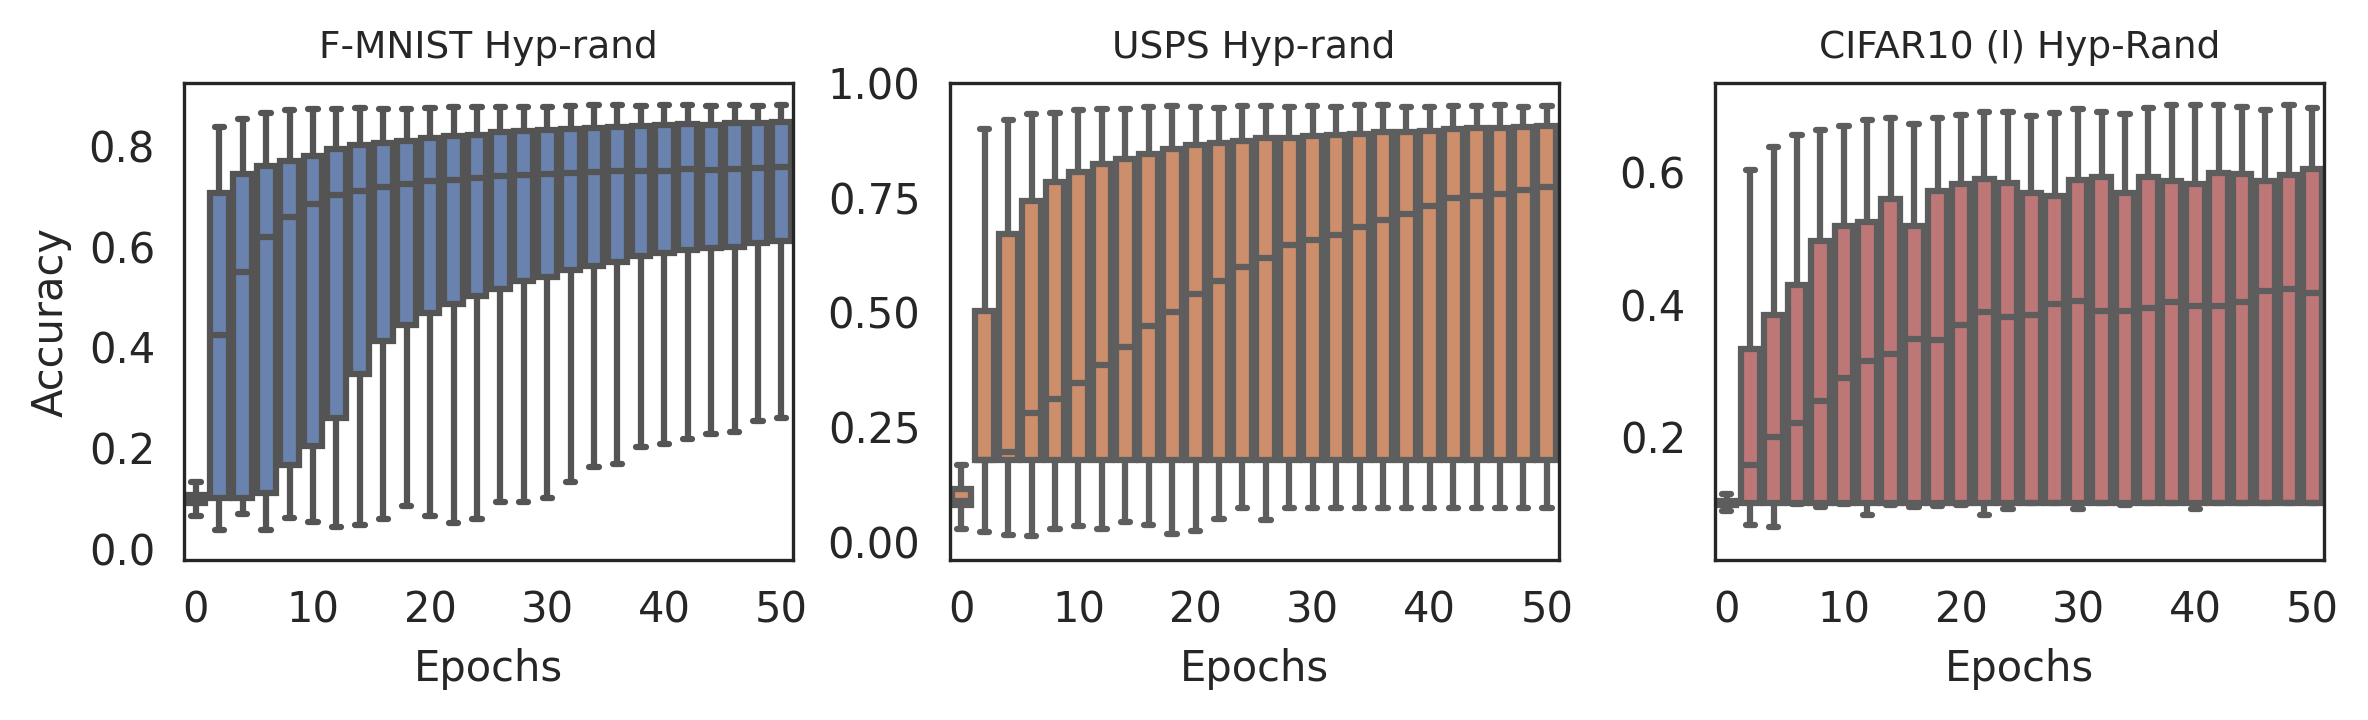
\includegraphics[trim=0in 0in 0in 0in, width=0.85\linewidth]{imgs/boxplots_mix.png}
\vspace{-8pt}
\caption{
Accuracy distribution over epochs for the \texttt{F-MNIST Hyp-rand}, \texttt{USPS Hyp-rand} and \texttt{CIFAR Hyp-rand} zoos. All zoos show training progress and considerable performance diversity.\looseness-1
}
\vspace{-10pt}

\label{fig:boxplots}    
\end{center}
\end{minipage}
\end{figure}


%%%%%%%%%%%%%%%%%%%%%%%%%%%%%%%%%%%%%%%%%%%%%%%%%%%%%%
%
%   training protocol
%
%%%%%%%%%%%%%%%%%%%%%%%%%%%%%%%%%%%%%%%%%%%%%%%%%%%%%%
\subsection{Training of Model Zoos}
\vspace{-4pt}
Neural network models are trained from the previously defined three configurations 
$\{\mathcal{D}, \lambda, \mathcal{A}\}$ (Seed, Hyp-10-rand, Hyp-10-fix, see Sec 2.1). With the \textit{8 image datasets} and the three configurations, 
this results in \textit{27 model zoos}.
%
% 47'360
%  2’415’360 collected model states. 
%
% The zoos include a total of around \textit{47'360} unique neural networks, each trained fo 50 epochs. 
% This makes 51 checkpoints per model training trajectory including the starting checkpoint 
% representing the model initialization before training starts. In total, this results in a set of 
% approx. \textit{2’415’360} collected model states. 
The zoos include a total of around \textit{50'360} unique neural network models.\looseness-1

\textbf{Training Protocol:}
Every model in the collection of zoos is trained according to the same protocol. 
We keep the same train, validation and test splits for each zoo, and train each model for 50 epochs with gradient descent methods (SGD+momentum or ADAM). 
At every epoch, the model checkpoint as well as accuracy and loss of all splits are recorded. 
Validation and test performance are also recorded before the first training epoch.
This makes 51 checkpoints per model training trajectory including the starting checkpoint 
representing the model initialization before training starts. 
The ResNet-18 zoos on CIFAR100 and Tiny Imagenet require more updates and are trained for 60 epochs.
In total, this results in a set of \textit{2’585’360} collected model states.\looseness-1


\textbf{Splits:}
To enable comparability, this set of models is split into \texttt{training} (70\%), \texttt{validation} (15\%), and \texttt{test} (15\%) subsets. 
This split is done such that all individual checkpoints of one model training (i.e., the 51 checkpoints per training) 
is entirely in either \texttt{training}, \texttt{validation}, or \texttt{test} and therefore no information is leaked between these subsets.\looseness-1

\textbf{Sparsified Model Zoo Twins:}
Model sparsification is an effective method to reduce computational cost of models. 
However, methods to sparsify models to a high degree while preserving the performance are still actively researched~\citep{hoeflerSparsityDeepLearning2021}. 
In order to allow systematic studies of sparsification, we are extending the model zoos with sparsified \textit{model zoo twins} serving as counterparts to existing zoos in the dataset. Using Variational Dropout (VD)~\citep{molchanovVariationalDropoutSparsifies2017}, we sparsify the trained models from existing model zoos. VD generates a sparsification trajectory for each model, along which we track the performance, degree of sparsity and the sparsified checkpoint. With 25 sparsification epochs, this yields 1'259'000 sparsification model states.

%
%
%
%
%
%%%%%%%%%%%%%%%%%%%%%%%%%%%%%%%%%%%%%%%%%%%%%%%%%%%%%%
%
%   training protocol
%
%%%%%%%%%%%%%%%%%%%%%%%%%%%%%%%%%%%%%%%%%%%%%%%%%%%%%%
\subsection{Data Management and Accessibility of Model Zoos}
\label{sec:data_management}
The model zoos are made publicly available in an accessible, standardized, and well documented way to the research community under the Creative Commons Attribution 4.0 license (CC-BY 4.0). 
We ensure the technical accessibility of the data by hosting it on Zenodo, where the data will be hosted for at least 20 years.
Further, we take steps to reduce access barriers by providing code for data loading and preprocessing, to reduce the friction associated with analyzing of the raw zoo files.
All code can be found on the model zoo website \href{www.modelzoos.cc}{www.modelzoos.cc}.
To ensure conceptional accessibility, we include detailed insights, visualizations and the analysis of the model zoo (Sec. \ref{sec:analysis}) with each zoo.
Further details can be found in Appendix \ref{app:data_management}.\looseness-1 
%

%
%
%
